\epigraph{Eine Theorie ohne testbare Vorhersagen ist Philosophie. T0 liefert Zahlen.}{}

Eine physikalische Theorie muss sich messen lassen --- buchstäblich. Die T0-Theorie macht eine Reihe konkreter, quantitativer Vorhersagen, die mit heutiger oder naher zukünftiger Technologie überprüfbar sind.

\section{Bell-Test-Abweichungen}


\begin{figure}[htbp]
\centering
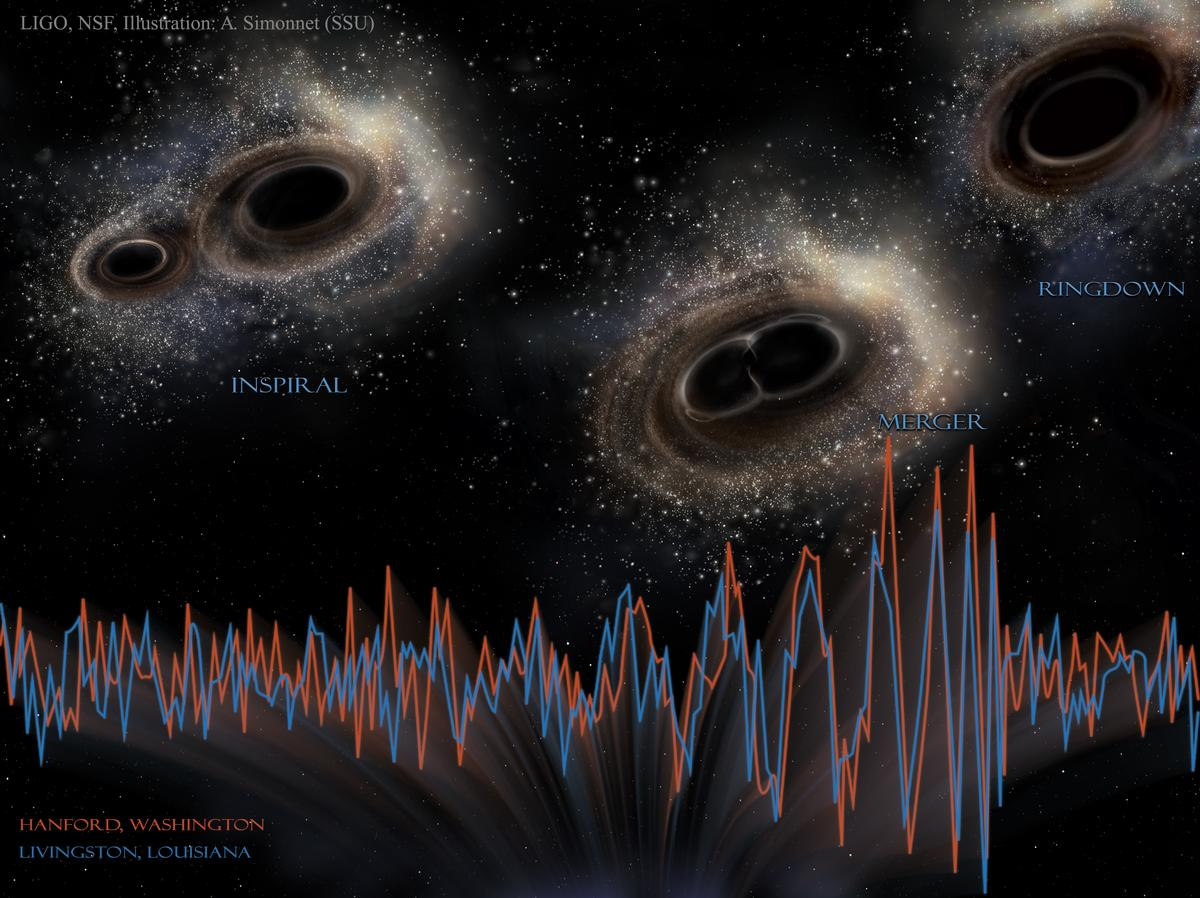
\includegraphics[width=0.85\textwidth]{img/ligo_gw_big.jpg}
\caption{GW150914 (LIGO): Zwei verschmelzende Schwarze Löcher --- Inspiral, Merger, Ringdown. T0 sagt Korrekturen bei hohen Frequenzen voraus. Credit: LIGO, NSF; Illustration: A.~Simonnet (SSU).}
\end{figure}
Die T0-modifizierten Bell-Ungleichungen sagen Abweichungen der Größenordnung~$\sim 10^{-3}$ in Multi-Qubit-Systemen voraus. Die Wahl von 73~Qubits als Benchmark ergibt sich aus der Analyse in \href{https://github.com/jpascher/T0-Time-Mass-Duality/blob/main/2/pdf/142_Experimet-verschraenkung_De.pdf}{Dok.~142}: Bei dieser Systemgröße wird die kumulative $\xsi$-Korrektur an den CHSH-Korrelationen erstmals systematisch messbar, während das System noch experimentell kontrollierbar bleibt.

\section{Räumliche Korrelationsverzögerungen}

Über große Distanzen sagt T0 messbare Verzögerungen in Verschränkungskorrelationen voraus. Die Abschätzung folgt aus $\Delta t \approx \xsi \cdot d/c$: Für $d = 1000$~km ergibt sich $\Delta t \approx 1{,}33 \times 10^{-4} \times 1000\,\text{km} / c \approx 445$~Nanosekunden (\href{https://github.com/jpascher/T0-Time-Mass-Duality/blob/main/2/pdf/020_T0_QM-QFT-RT_De.pdf}{Dok.~020}). Dies wäre in einem Satellitenexperiment --- vergleichbar mit dem chinesischen Micius-Experiment, aber mit höherer Zeitauflösung --- nachweisbar.

\section{Quantencomputer-Fehlerraten}

Die T0-Korrektur an Quantencomputer-Fehlerraten ist systematisch:
\begin{equation}
\varepsilon_{\text{T0}} = \varepsilon_{\text{Standard}} \cdot \left(1 - \xsi \cdot \frac{E_{\text{gate}}}{E_{\text{Planck}}}\right)
\end{equation}

Die Korrektur ist winzig, aber \emph{systematisch} --- sie sollte sich als konsistente Abweichung von den Standardvorhersagen in großen Quantenschaltkreisen zeigen.

\section{Atominterferometrie}

Atominterferometer der neuesten Generation erreichen Empfindlichkeiten, die T0-Korrekturen zugänglich machen. Die vorhergesagte Phasenverschiebung beträgt~$\sim 10^{-18}$~Radiant --- am Rande des aktuell Messbaren, aber innerhalb der Reichweite geplanter Experimente.

\section{Gravitationswellen-Korrekturen}

Die LIGO/Virgo-Observatorien messen Gravitationswellen mit beispielloser Präzision. T0 sagt Korrekturen in den Wellensignalen bei hohen Frequenzen voraus --- dort, wo die fraktale Struktur der Raumzeit sich am stärksten bemerkbar macht.

\begin{figure}[htbp]
\centering
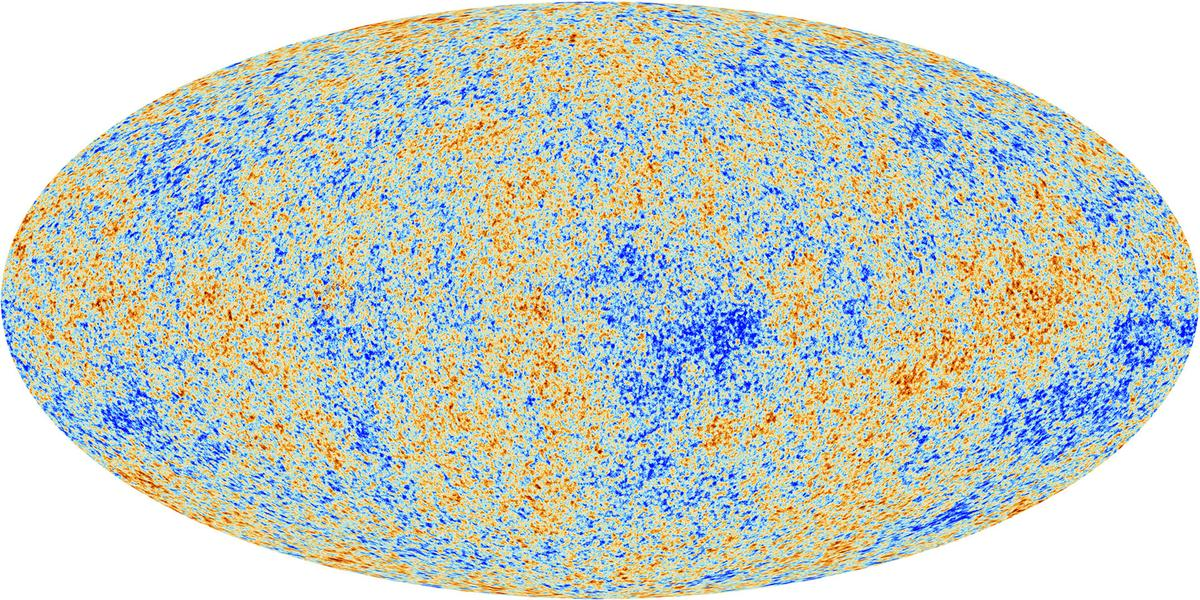
\includegraphics[width=\textwidth]{img/planck_cmb_final.jpg}
\caption{Die kosmische Mikrowellenhintergrundstrahlung (CMB), beobachtet vom Planck-Satelliten. In T0 entstehen die Anisotropien durch Zeitfeldvariationen --- nicht durch inflationäre Expansion. Credit: ESA und die Planck-Kollaboration.}
\end{figure}

\section{Die Tau-Anomalie}

Eine besonders scharfe Vorhersage betrifft das anomale magnetische Moment des Tau-Leptons:
\begin{equation}
a_\tau \approx 1{,}282 \times 10^{-3}
\end{equation}

Diese Vorhersage ist testbar am Belle~II-Experiment in Tsukuba, Japan. Ein bestätigter Wert wäre ein starkes Indiz für die T0-Geometrie.

\begin{zusammenfassung}
T0 ist keine rein theoretische Konstruktion. Die Theorie macht mindestens ein halbes Dutzend quantitative Vorhersagen, die mit existierender oder geplanter Experimentaltechnologie überprüfbar sind. Die Natur wird entscheiden.
\end{zusammenfassung}
